\section{Evaluation}
\label{sec:Evaluation}
This section contains the evaluation and the graphical representation of the measurements. The following subsections contain the measurement results of the individual tasks listed in chapter \ref{subsec:Measurements}. The aim is to determine the sound velocity and the attenuation coefficient of different materials. The exact descriptions of the tasks can be found in the assignment \cite{ultrasound}.

%-----------------------------------------------------------------------------------
\subsection{Wave Length Calculation}
\label{subsec:wave_length_calculation}
The following table \ref{tab:wave_length_calculation} shows the calculated wave length $\lambda$ of the ultrasound wave in air, distilled water and aluminium at 1 kHz, 1 MHz and 5 MHz. All literature longitudinal sound velocities are at 20 \textdegree C room temperature.

\begin{table}[H]
	\centering
	\renewcommand{\arraystretch}{1.3}
	\begin{tabular}{r||c|c|c|c}
		& $\boldsymbol{c_L}$ ($\frac{\si{m}}{\si{s}}$) \cite{kohlrausch} & $\boldsymbol{\lambda}$ \textbf{@ 1 kHz} (m) & $\boldsymbol{\lambda}$ \textbf{@ 1 MHz} (m) & $\boldsymbol{\lambda}$ \textbf{@ 5 MHz} (m) \\
		\hline\hline
		\textbf{Air} & 344 & 0.34 & $344\cdot 10^{-6}$ & $68.8\cdot 10^{-6}$ \\
		\textbf{Distilled Water} & 1483 & 1.48 & $1.48\cdot 10^{-3}$ & $297\cdot 10^{-6}$ \\
		\textbf{Aluminium} & 6400 & 6.40 & $6.40\cdot 10^{-3}$ & $1.28\cdot 10^{-3}$ \\
	\end{tabular}
	\caption{Calculated wave lengths $\lambda$ for different solids and liquids at the audible frequency 1 kHz and the two ultrasound frequencies 1 MHz and 5 MHz. The calculations were carried out in the software Microsoft Office Excel.}
	\label{tab:wave_length_calculation}
\end{table}

%-----------------------------------------------------------------------------------
\subsection{Longitudinal Ultrasound Velocities in Solids}
\label{subsec:Longitudinal_Ultrasound_Velocities_in_Solids}
Table \ref{tab:Longitudinal_Ultrasound_Velocities_in_Solids} shows the calculated longitudinal ultrasound velocities from the measurements. These results were obtained using linear regression. This was done in the software QtiPlot. To use linear regression, equation \ref{eq:sound_velocity} has to be rearranged, so that it relates the time of flight with the distance and an offset $b$ has to be added:

\begin{equation}
\Delta t = \frac{2x}{c_L} + b
\label{eq:sound_velocity_linear_regression}
\end{equation}

This equation \ref{eq:sound_velocity_linear_regression} can now be used in QtiPlot.

\begin{table}[H]
	\centering
	\renewcommand{\arraystretch}{1.3}
	\begin{tabular}{r||c|c|c}
		& $\boldsymbol{c_L}$ \textbf{@ 1 MHz} ($\frac{\si{m}}{\si{s}}$) & $\boldsymbol{c_L}$ \textbf{@ 5 MHz} ($\frac{\si{m}}{\si{s}}$) & \textbf{Literature Value} ($\frac{\si{m}}{\si{s}}$) \cite{kohlrausch} \\
		\hline\hline
		\textbf{PMMA} & $(2751\pm 5)$ & $(2721\pm 10)$ & $\approx 2700$ \\
		\textbf{Aluminium} & - & $(6387\pm 30)$ & $\approx 6400$ \\
		\textbf{Copper} & - & $(4680\pm 17)$ & $\approx 4700$ \\
		\textbf{Brass} & - & $(4627\pm 46)$ & $\approx 4700$ \\
	\end{tabular}
	\caption{Measured longitudinal ultrasound velocities $c_L$ in different solids. Furthermore, the literature value of $c_L$ is stated. The literature values are from a physics book from 1968.}
	\label{tab:Longitudinal_Ultrasound_Velocities_in_Solids}
\end{table}

The longitudinal ultrasound velocities of the metals could not be measured with a frequency of 1 MHz. Figure \ref{fig:ghost} shows the measured \flqq ghost signals\frqq\ (signals which are overlapping). Due to this, the longitudinal ultrasound velocities of the metals was only measured with a frequency of 5 MHz, which works perfectly fine.

Figures \ref{fig:Longitudinal_Ultrasound_Velocity_of_PMMA} and \ref{fig:Longitudinal_Ultrasound_Velocity_of_Aluminium} show the plots obtained from QtiPlot for PMMA and aluminium respectively.

\begin{figure}[H]
	\centering
	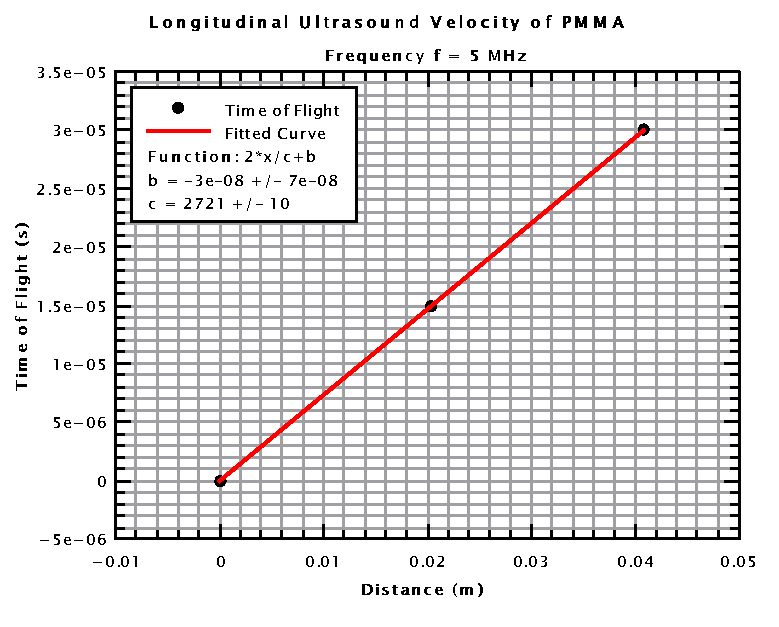
\includegraphics[scale=0.94]{Longitudinal_Ultrasound_Velocity_of_PMMA}
	\caption{This plot shows the time of flight $\Delta t$ in relation to the distance $x$ for PMMA.Linear regression can then be used on these discrete values to obtain the longitudinal ultrasound velocity of PMMA. The fitted curve is shown in red and the discrete measurements are shown as black dots.}
	\label{fig:Longitudinal_Ultrasound_Velocity_of_PMMA}
\end{figure}

\begin{figure}[H]
	\centering
	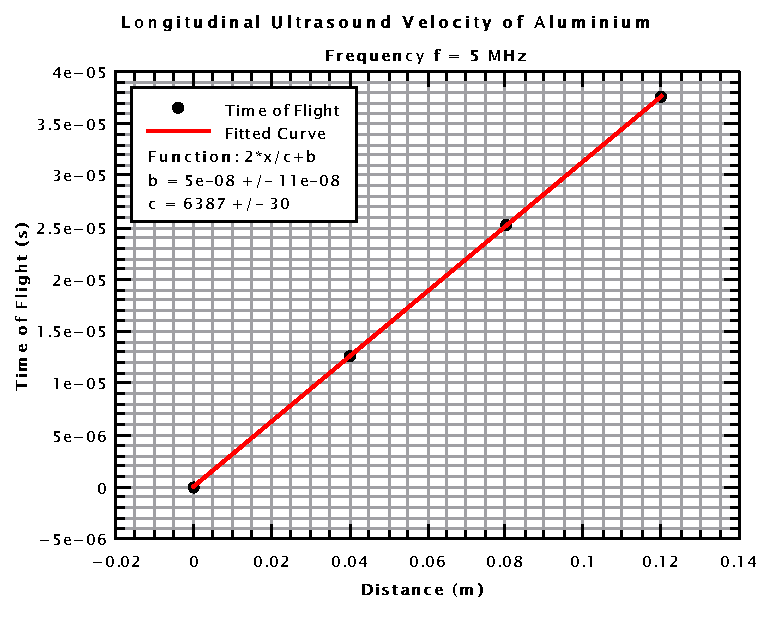
\includegraphics[scale=0.94]{Longitudinal_Ultrasound_Velocity_of_Aluminium}
	\caption{Linear regression is used here as well. This time to obtain the longitudinal ultrasound velocity of aluminium. The measurement had to be done at a frequency of 5 MHz because of ghost signals (see figure \ref{fig:ghost}). The fit is shown in red and the measurements as black dots.}
	\label{fig:Longitudinal_Ultrasound_Velocity_of_Aluminium}
\end{figure}

\begin{figure}[H]
	\centering
	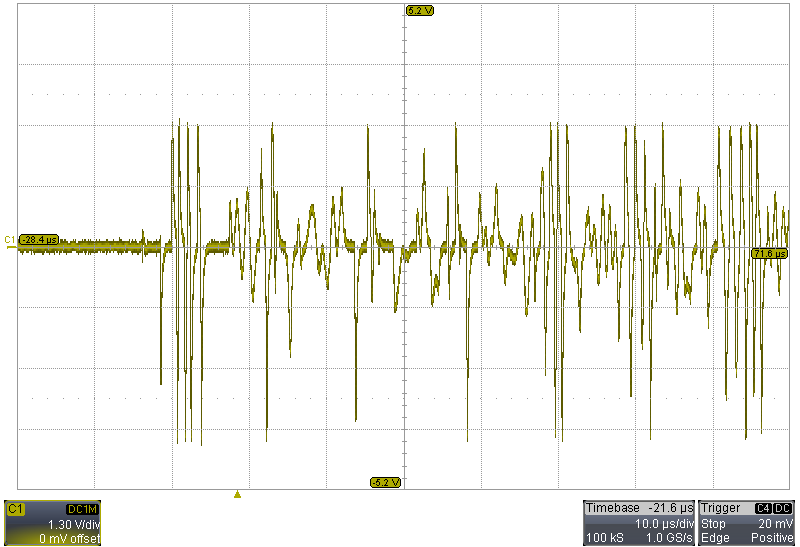
\includegraphics[scale=0.5]{ghost}
	\caption{When metals are measured with a transducer that has an oscillation frequency of 1~MHz, \flqq ghost signals\frqq\ occur. This is due to the much higher longitudinal ultrasound velocity of the metals, which leads to signals overlapping also known as \flqq ghost signals\frqq. To get rid of this effect the oscillation frequency can be increased.}
	\label{fig:ghost}
\end{figure}

\newpage
%-----------------------------------------------------------------------------------
\subsection{Attenuation Coefficient of PMMA}
\label{subsec:Attenuation_Coefficient_of_PMMA}
The results for the attenuation coefficient $\mu$ of PMMA are shown in table \ref{tab:Attenuation_Coefficient_of_PMMA} below. The attenuation coefficient $\mu$ was measured with an oscillation frequency of 1 MHz and 5 MHz.

\begin{table}[H]
	\centering
	\renewcommand{\arraystretch}{1.3}
	\begin{tabular}{r||c|c}
		& $\boldsymbol{\mu}$ \textbf{@ 1 MHz} ($m^{-1}$) & $\boldsymbol{\mu}$ \textbf{@ 5 MHz} ($m^{-1}$) \\
		\hline\hline
		\textbf{PMMA} & $(16\pm 1)$ & $(43\pm 3)$ \\
	\end{tabular}
	\caption{Results of the non-linear fit carried out in the software QtiPlot. The unit of the attenuation coefficient $\mu$ has to be m$^{-1}$ due to the fact, that the exponent of $e$ has to be uniform and the distance has the unit m. This leads to the following: $\si{m}^{-1}\cdot \si{m} = 1$.}
	\label{tab:Attenuation_Coefficient_of_PMMA}
\end{table}

To obtain these results, non-linear regression was used. The necessary exponential relationship of the absorption is shown in equation \ref{eq:absorption}. This relationship was used in QtiPlot to create the fit shown in figure \ref{fig:Attenuation_Coefficient_of_PMMA}.

\begin{figure}[H]
	\centering
	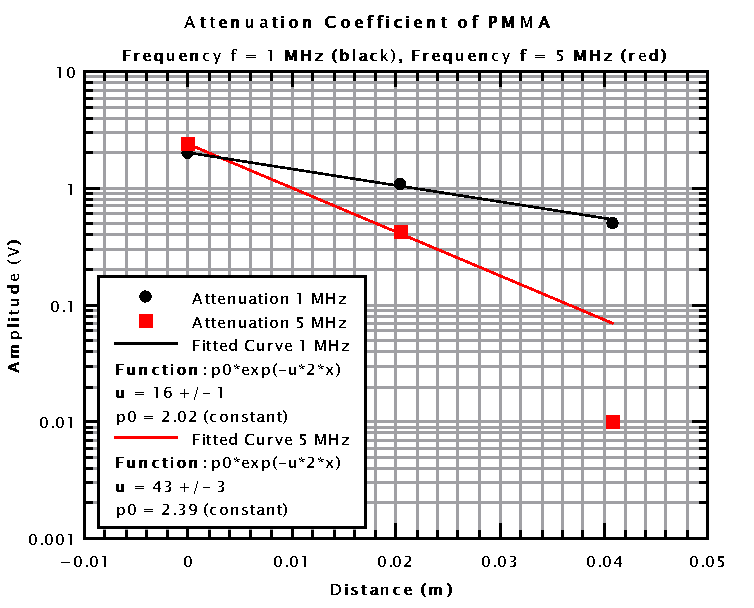
\includegraphics[scale=1]{Attenuation_Coefficient_of_PMMA}
	\caption{Semi-log plot of the amplitude $A$ in function of the distance $x$ which shows the attenuation of the signal in PMMA. The black and red line represent the exponential fit of the attenuation. The fits look like a linear function because of the logarithmic y-axis. Furthermore, the attenuation at a lower frequency is less than at a higher frequency, just as expected (see chapter \ref{subsec:Absorption}). Noticeable is the last red measurement value which seems to be off by quite a bit. This is probably due to the small amplitude which leads to measurement inaccuracies.}
	\label{fig:Attenuation_Coefficient_of_PMMA}
\end{figure}

\newpage
%-----------------------------------------------------------------------------------
\subsection{Longitudinal Ultrasound Velocities in Liquids}
\label{subsec:Longitudinal_Ultrasound_Velocities_in_Liquids}
Table \ref{tab:Longitudinal_Ultrasound_Velocities_in_Liquids} shows the results of the fits obtained from QtiPlot. The longtidunial ultrasound velocities $c_L$ differ quite bit from each other. In other words, the temperature of a liquid such as water is not negligible when doing calculations with sound waves.

\begin{table}[H]
	\centering
	\renewcommand{\arraystretch}{1.3}
	\begin{tabular}{r||c|c}
		& $\boldsymbol{c_L}$ \textbf{@ 5 MHz} ($\frac{\si{m}}{\si{s}}$) & \textbf{Literature Value} ($\frac{\si{m}}{\si{s}}$) \cite{kohlrausch} \\
		\hline\hline
		\textbf{Water 21 \textdegree C} & $(1488\pm 3)$ & $\approx 1483$ \\
		\textbf{Water 49 \textdegree C} & $(1538\pm 5)$ & $\approx 1540$ \\
		\textbf{Saltwater 40 \textdegree C} & $(1612\pm 6)$ & $\approx 1620$ \\
	\end{tabular}
	\caption{Measured longitudinal ultrasound velocities $c_L$ in water and saltwater at different temperatures. The saltwater has a salt concentration of approx. 10 \% (90 g salt / 0.901 L). Furthermore, the literature value of $c_L$ is stated.}
	\label{tab:Longitudinal_Ultrasound_Velocities_in_Liquids}
\end{table}

Figure \ref{fig:Longitudinal_Ultrasound_Velocity_of_Water} shows an example plot from QtiPlot for destilled water with a temperature of 21 \textdegree C. Solely an oscillation frequency of 5 MHz was used to obtain all measurements.

\begin{figure}[H]
	\centering
	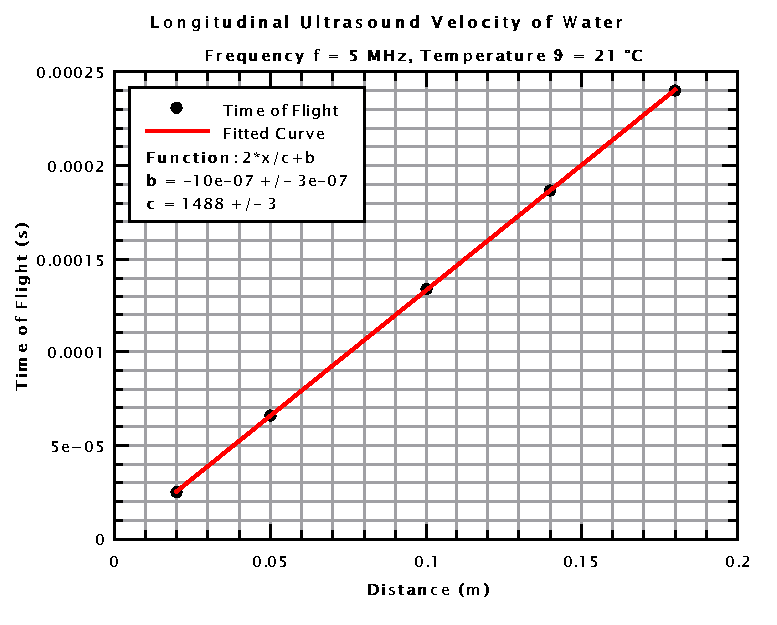
\includegraphics[scale=1]{Longitudinal_Ultrasound_Velocity_of_Water}
	\caption{This plot shows the linear fit and the discrete measurement values for destilled water with a temperature of 21 \textdegree C. The time of flight was measured in function of the travelled distance. The measurements were taken with no linear relationship to each other (not always the same $\Delta x$ between to meassured values). The statistical error is quite low, which means the measured values must match each other really well.}
	\label{fig:Longitudinal_Ultrasound_Velocity_of_Water}
\end{figure}

\newpage
%-----------------------------------------------------------------------------------
\subsection{Transversal Ultrasound Velocity in PMMA}
\label{subsec:Transversal_Ultrasound_Velocity_in_PMMA}
A special transversal transducer was used to measure the transverse time of flight of a sound wave in PMMA. An oscillation frequency $f$ of 1 MHz was used to obtain the measurement results. Table \ref{tab:Transversal_Ultrasound_Velocity_in_PMMA} shows the calculated transversal ultrasound velocity $c_T$ for PMMA.

\begin{table}[H]
	\centering
	\renewcommand{\arraystretch}{1.3}
	\begin{tabular}{r||c|c}
		& $\boldsymbol{c_T}$ \textbf{@ 1 MHz} ($\frac{\si{m}}{\si{s}}$) & \textbf{Literature Value} ($\frac{\si{m}}{\si{s}}$) \cite{kohlrausch} \\
		\hline\hline
		\textbf{PMMA (Transversal)} & $(1405\pm 14)$ & $\approx 1350$ \\
	\end{tabular}
	\caption{To measure the transversal time of flight, a special kind of ultrasound shear gel had to be used in conjunction with a special transducer. The transducer was manufactured to be used at an oscillation frequency of 1 MHz.}
	\label{tab:Transversal_Ultrasound_Velocity_in_PMMA}
\end{table}

Only two measurments were obtained, but it is possible to use $0$ as another measurement value. This is due to the fact that at a distance of $0$ the time of flight will always be $0$ as well. Figure \ref{fig:Transversal_Ultrasound_Velocity_of_PMMA} shows the plot obtained from QtiPlot.

\begin{figure}[H]
	\centering
	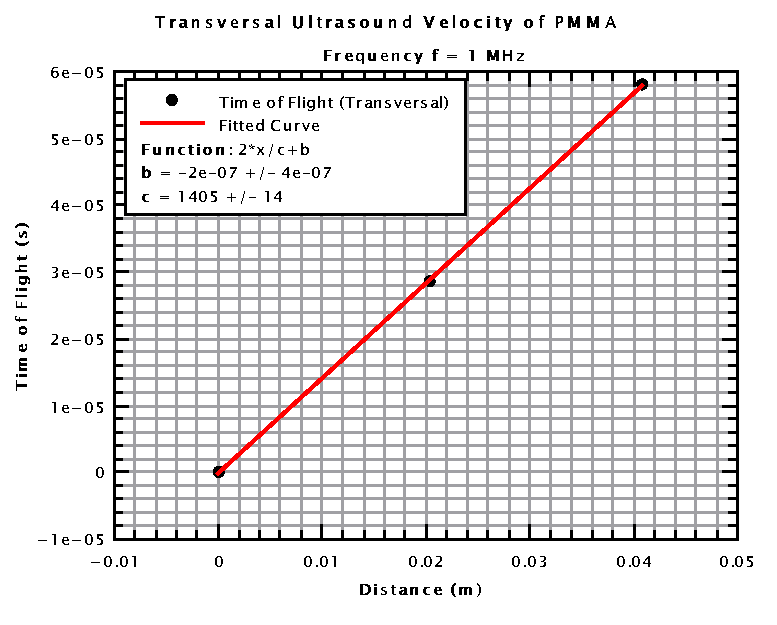
\includegraphics[scale=1]{Transversal_Ultrasound_Velocity_of_PMMA}
	\caption{Measurement values of the transversal time of flight $\Delta t$ in PMMA in function of the distance $x$. With only two measurement values QtiPlot obviously can not calculate the statistical error. Due to this, an additional measurement value at a distance of $0$ m was set to $0$ s. Furthermore, linear regression was used to fit the red linear function.}
	\label{fig:Transversal_Ultrasound_Velocity_of_PMMA}
\end{figure}
